\chapter{Demo-Anwendung im Browser}
\label{cha:DemoAnwendung}

Um die praktische Anwendung von MiniJava für typische Browser"=Anwendungen zu demonstrieren, wurde eine einfache Web"=Anwendung implementiert, die Fibonacci"=Zahlen berechnen kann.

\section{Anforderungen an den Fibonacci-Rechner}
Die Benutzeroberfläche (siehe Abbildung \ref{fig:fibCalculatorBrowser} auf Seite \pageref{fig:fibCalculatorBrowser}) soll zwei Eingabefelder (für die Werte $a$ und $b$) und einen Start"=Knopf darstellen. Beim Drücken des Start"=Knopfs soll die Anwendung die Fibonacci"=Zahlen von $fib(a)$ bis $fib(b)$ berechnen und in einer Tabelle ausgeben.

Der Fokus des Fibonacci"=Rechners liegt darauf, MiniJava in einem abgeschlossenen Projekt zu präsentieren und zu zeigen, wie MiniJava mit dem Browser interagieren kann. Dabei wurde der Aspekt einer effizienten Implementierung bewusst vernachlässigt. Dadurch wirken zwar einige Quelltext"=Abschnitte erzwungen (beispielsweise das rekursive Berechnen jeder einzelnen Fibonacci-Zahl ohne Speichern von Zwischenergebnissen oder das Kapseln von Methodenparametern in Objekte), gleichzeitig wird dadurch aber ermöglicht, im Rahmen eines überschaubaren Anwendungsfalls möglichst viele Funktionalitäten von MiniJava einzusetzen.

Zum Vergleich wurden dieselben Anforderungen zur Gänze auch in JavaScript implementiert. Ziel ist dabei lediglich ein Vergleich zwischen den Programmiersprachen und nicht eine idente oder gar deckungsgleiche Implementierung.

In diesem Kapitel werden nur relevante Quelltext"=Ausschnitte gezeigt.

\pagebreak
\section{Implementierung in MiniJava}

Nachfolgend findet sich die Implementierung des Fibonacci"=Rechners in MiniJava.
\lstinputlisting{src/demoAnwendung/ClickEventListener.minijava}
\pagebreak
\lstinputlisting{src/demoAnwendung/FibonacciCalculator.minijava}
\lstinputlisting{src/demoAnwendung/Main.minijava}

\section{Implementierung in JavaScript}

Nachfolgend findet sich die Implementierung des Fibonacci"=Rechners in JavaScript.
\lstinputlisting{src/demoAnwendung/js-version.js}

\section{Build-Prozess und Ausführen der Web-Anwendung}

Ähnlich wie bei der Konsolenanwendung im vorherigen Kapitel wird hier ebenfalls Gradle eingesetzt, um den MiniJava"=Quelltext zu kompilieren. Zusätzlich dazu wird webpack \cite{Webpack} eingesetzt, um alle JavaScript"=Dateien in eine einzige JavaScript"=Datei zusammenzufassen. Sämtliche \lstinline{require}"=Referenzierungen werden dabei aufgelöst.

Zusätzlich zur Basis"=Standardbibliothek wird eine eigene für den Browser mitkompiliert. Diese enthält Funktionalitäten, die auf Browser"=Schnittstellen abgebildet werden (Implementierungsdetails sind im nächsten Abschnitt zu finden).

Beim Ausführen muss sichergestellt werden, dass das binäre WebAssembly"=Modul vom Web"=Server mit dem MIME"=Type \lstinline{application/wasm} bereitgestellt wird, sonst kann es zu Laufzeitfehlern kommen \cite{MDNWebAssembly}. Zu Entwicklungs- und Testzwecken reicht dafür das NPM"=Modul \lstinline{lite-server}\footnote{\url{https://www.npmjs.com/package/lite-server}} vollkommen aus. Für den produktiven Einsatz sollte man diesen Aspekt bei der Konfiguration des Web"=Servers beachten. Im Git"=Repository findet sich eine lauffähige Konfiguration für den Apache HTTP Server in Form eines \emph{Dockerfiles}.

\section{Auszug aus der Standardbibliothek für den Browser}

Um in MiniJava sinnvoll mit dem Browser interagieren zu können, wurde eine kleine Standardbibliothek entwickelt. Zwei Funktionen daraus werden nun im Detail betrachtet: Das Abfragen eines HTML"=Knotens aus dem DOM über die ID des Elements und das Hinzufügen eines Event"=Listeners für das Mausklick"=Ereignis zu einem HTML"=Knoten. In der Standardbibliothek sind noch weitere Methoden zur Modifikation des DOMs vorhanden, unter anderem das Erstellen und Einfügen von Knoten.

\lstinputlisting{src/demoAnwendung/Browser.minijava}
\lstinputlisting{src/demoAnwendung/Browser.js}

Nachfolgend einige Details zum JavaScript"=Teil der beiden Methoden:

Mit der Funktion \lstinline{runtime.wasmRef} können DOM"=Knoten, welche die JavaScript"=Funktion \lstinline{document.getElementById} zurückgibt, MiniJava zugänglich gemacht werden.

Als Event"=Listeners für das Mausklick"=Eregnis wird eine JavaScript"=Funktion (Lambda"=Ausdruck) registriert. Diese Funktion delegiert das Ereignis an das beim Registrieren übergebene \lstinline{handler}"=Objekt. Dabei wird angenommen, dass in der Klasse dieses Objekts eine Methode namens \lstinline{handleEvent} existiert, die einen Parameter vom Typ \lstinline{MouseEvent} annimmt. Sollte so eine Methode nicht existieren, kommt es zu einem Laufzeitfehler.

\section{Ergebnis}

In Abbildung \ref{fig:fibCalculatorBrowser} sind zwei Bildschirm"=Schnappschüsse des Fibonacci"=Rechners im Browser. Links wurde die JavaScript"=Version ausgeführt, rechts die MiniJava"=Version. Man erkennt bei den ersten Zahlen, dass diese korrekt berechnet wurden.

\begin{figure}[]
    \centering
    \begin{tabular}{c c}
        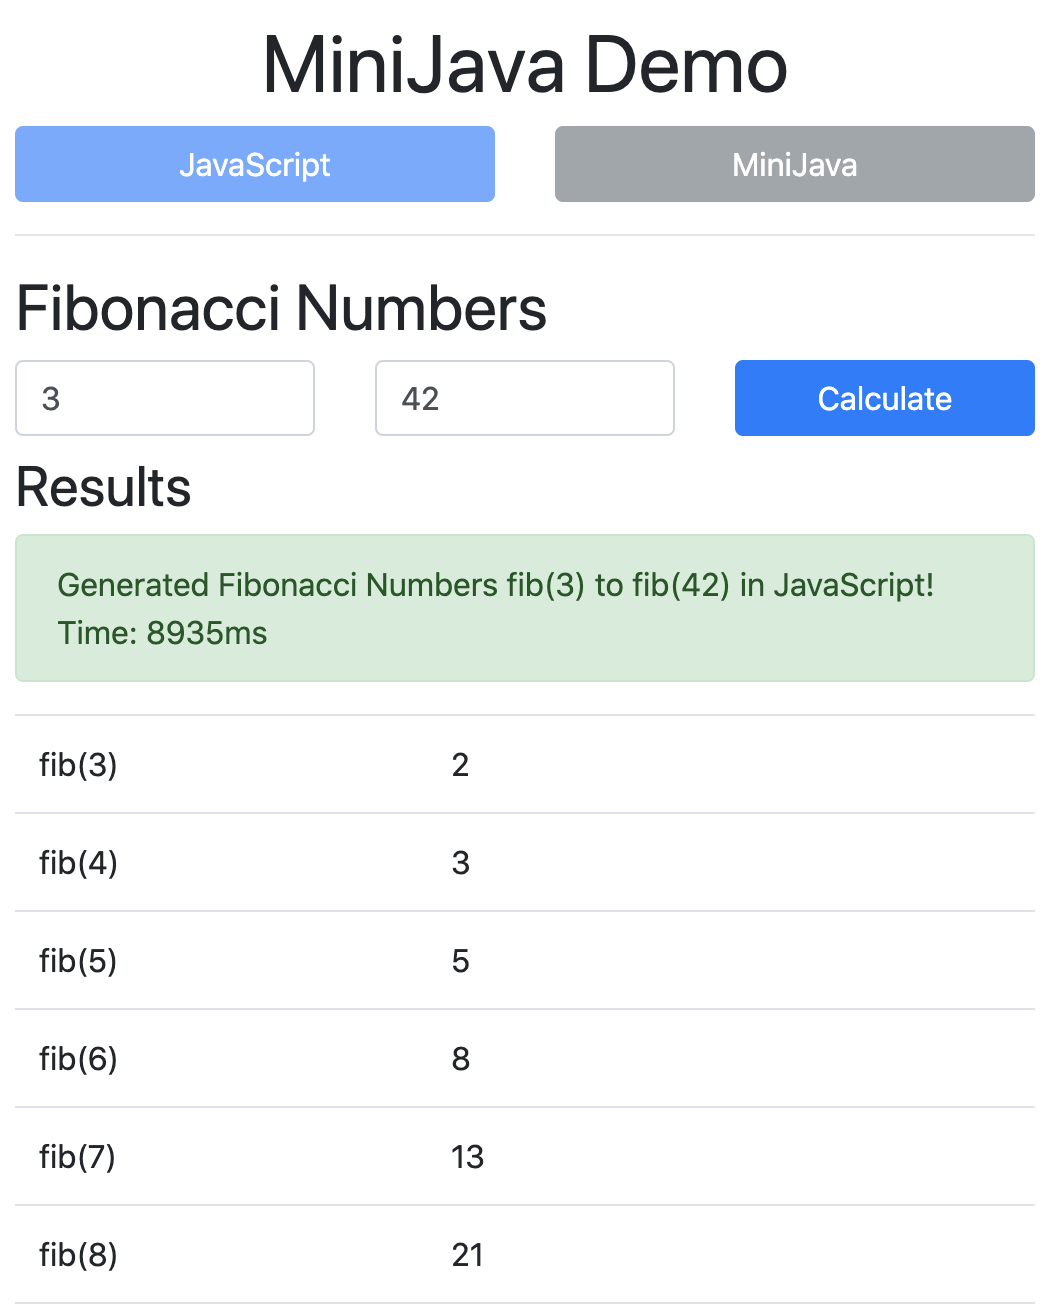
\includegraphics[width=0.47\textwidth]{demoAnwendung/fibonacciJavaScript} & 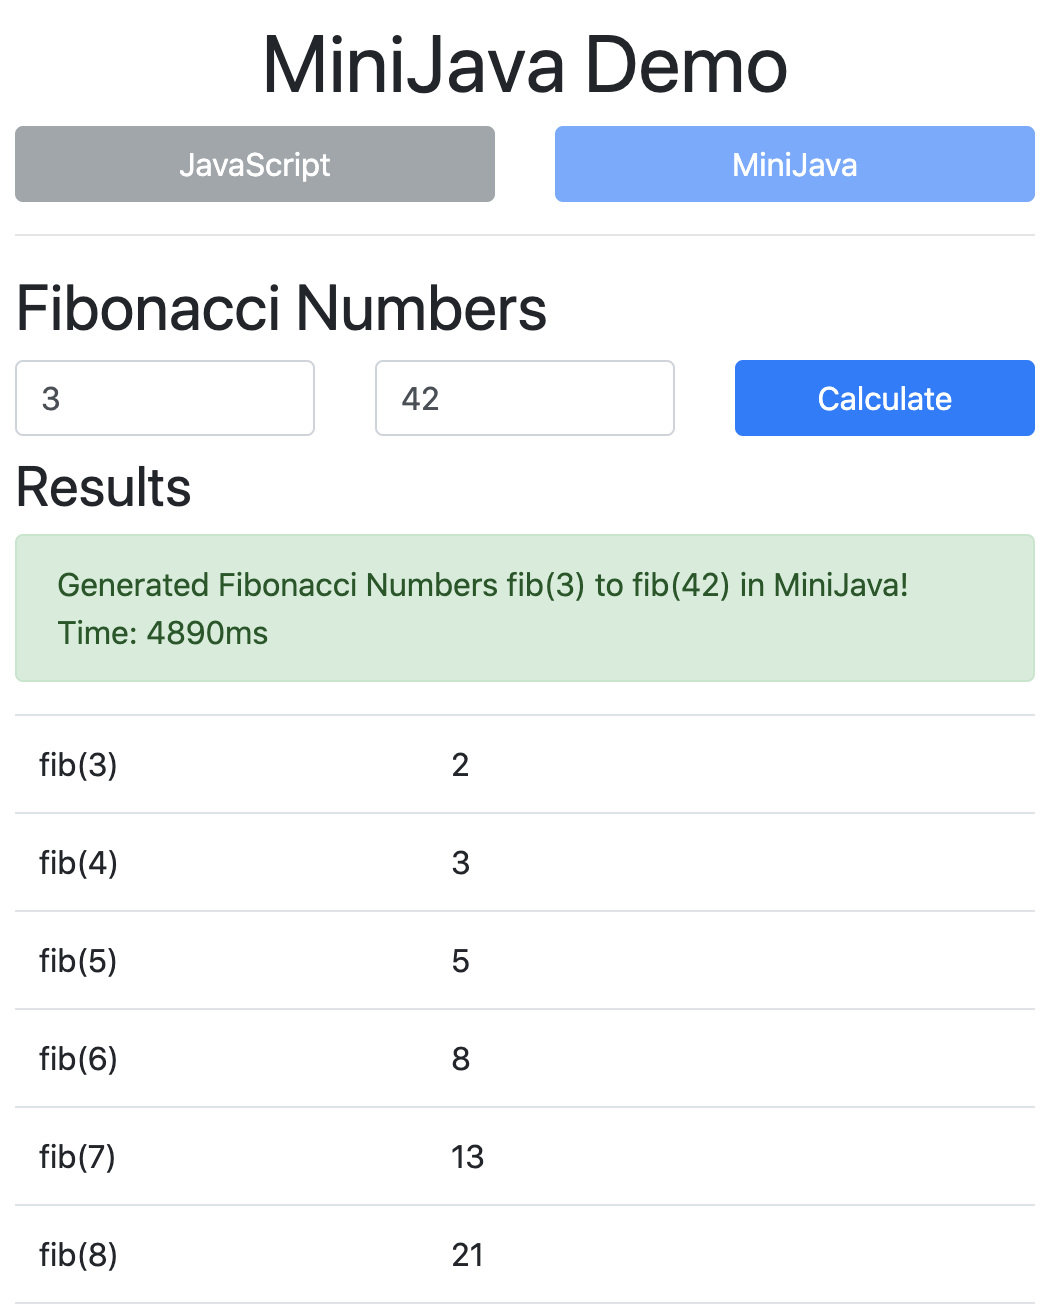
\includegraphics[width=0.47\textwidth]{demoAnwendung/fibonacciMiniJava}
    \end{tabular}
    \caption{Fibonacci-Rechner im Browser}
    \label{fig:fibCalculatorBrowser}
\end{figure}

Während der Ausführung wurde die Laufzeit gemessen, dabei wird die gesamte Zeit ab dem Klicken des Start"=Knopfs bis zum Erstellen der Tabelle berücksichtigt. Man erkennt, dass die Laufzeit der MiniJava"=Version (4890 Millisekunden) im Vergleich zur JavaScript"=Version (8935 Millisekunden) deutlich kürzer ist.

Der Fibonacci"=Rechner wurde auf der folgenden Sofware- und Hardware"=Konfiguration getestet:
\begin{itemize}
    \item Browser: Google Chrome (Mac) 81.0.4044.122 64"=Bit
    \item Betriebssystem: macOS 10.15.4
    \item Hardware: MacBook Pro (15"=inch, 2018)
    \begin{itemize}
        \item CPU: 2,6 GHz 6"=Core Intel Core i7
        \item RAM: 16 GB 2400 MHz DDR4
    \end{itemize}
\end{itemize}

\section{Vergleich JavaScript und MiniJava}

Insgesamt sieht man, dass die Implementierungen aus Quelltextsicht sehr ähnlich sind. Sämtliche Anforderungen wurden von beiden Varianten erfüllt.

Die Quelltextmenge ist bei JavaScript deutlich geringer, da keine Datentypen deklariert werden müssen, sondern diese direkt verwendet werden können. Außerdem bietet JavaScript im Vergleich zu MiniJava mehr syntaktische Konstrukte wie beispielsweise die \lstinline{for}"=Schleife oder Lambda"=Ausdrücke. 

Der wesentliche Vorteil bei MiniJava ist die Typsicherheit, da sämtliche Zugriffe auf Objekte bereits beim Kompilieren überprüft werden und beispielsweise flüchtige Tippfehler früh erkannt werden. Bei der Typsicherheit gibt es eine einzige Ausnahme: das Aufrufen der \lstinline{handleEvent}"=Methode, da von der Standardbibliothek angenommen wird, dass diese Methode existiert. Würde man allerdings MiniJava um \emph{Interfaces} erweitern, könnte man dieses Problem lösen, da dann wieder der Compiler in der Lage wäre, die Anwesenheit von Methoden zu garantieren.

Anhand der Laufzeitmessungen sieht man, dass die MiniJava"=Variante deutlich schneller läuft. Dies ist vor allem auf den rechenintensivsten Teil, der rekursiven Berechnung für jede einzelne Zahl, des Programms zurückzuführen, der bei MiniJava ausschließlich in der virtuellen WebAssembly"=Maschine läuft. Die Laufzeiten verhielten sich über mehrere Aufrufe hintereinander bei beiden Varianten stabil.

\vspace{4em}
In diesem Kapitel wurde der praktische Einsatz von MiniJava anhand des Fibonacci"=Rechners demonstriert. Es wurde ebenfalls auf den Build"=Prozess und die Interaktion mit dem Browser eingangen. Dieselbe Anwendung wurde ebenfalls mit JavaScript implementiert. Die beiden Implementierungen wurden miteinander verglichen.
